\begin{activity} \label{A:10.5.3} The voltage $V$ (in volts) across a circuit is given by Ohm's Law: $V = IR$, where $I$ is the current (in amps) in the circuit and $R$ is the resistance (in ohms). Suppose we connect two resistors with resistances $R_1$ and $R_2$ in parallel as shown in Figure \ref{F:10.5.CR_Circuit}. The total resistance $R$ in the circuit is given by
\[R = \frac{1}{R_1} + \frac{1}{R_2}.\]
\begin{figure}[ht]
\begin{minipage}{4in}
        \ba
    \item Assume that the current and the resistances $R_1$ and $R_2$ are changing over time, $t$. Use the Chain Rule to write a formula for $\frac{dV}{dt}$.



    \item Suppose that, at some particular point in time, we measure the current to be 3 amps and that the current is increasing at $\frac{1}{10}$ amps per second, while resistance $R_1$ is 2 ohms and decreasing at the rate of 0.2 ohms per second and $R_2$ is 1 ohm and increasing at the rate of $0.5$ ohms per second. At what rate is the voltage changing at this point in time?



    \ea
\end{minipage} \hspace{0.2in}
\begin{minipage}{1.15in}
\begin{center}
\resizebox{!}{1.15in}{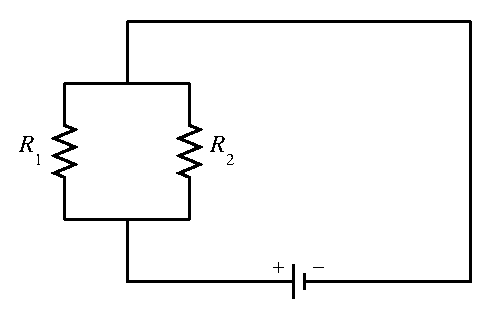
\includegraphics{10_5_CR_Circuit}}
\end{center}
\caption{Resistors in parallel.}
\label{F:10.5.CR_Circuit}
\end{minipage}
\end{figure}


\end{activity}
\begin{smallhint}

\end{smallhint}
\begin{bighint}

\end{bighint}
\begin{activitySolution}
\ba 
\item The voltage $V$ is a function of $I$, $R_1$, and $R_2$ as
\[V(I, R_1, R_2) = I\left(\frac{R_1+R_2}{R_1R_2}\right).\]
The Chain Rule tells us that 
\begin{align*}
\frac{dV}{dt} &= \frac{\partial V}{\partial I} \frac{dI}{dt} + \frac{\partial V}{\partial R_1} \frac{dR_1}{dt} + \frac{\partial V}{\partial R_2} \frac{dR_2}{dt}   \\
	&= \left(\frac{1}{R_1} + \frac{1}{R_2}\right) \frac{dI}{dt} - \left(\frac{I}{R_1^2}\right) \frac{dR_1}{dt} - \left(\frac{I}{R_2^2} \right) \frac{dR_2}{dt}.
\end{align*}

\item Given $I = 3$, $\frac{dI}{dt} = 0.1$, $R_1 = 2$, $\frac{dR_1}{dt} = -0.2$, $R_2 = 1$, and  $\frac{dR_2}{dt} = 0.5$, at this particular point in time we have 
\[\left. \frac{dV}{dt}\right|_{(3,2,1)} = \left(\frac{1}{2}+\frac{1}{1}\right) (0.1) - \left(\frac{3}{4}\right) (-0.2) - \left(\frac{3}{1} \right) (0.5) = -1.2 \ \frac{\text{Volts}}{\text{second}}.\]

\ea

 
\end{activitySolution}
\aftera